% !TEX TS-program = pdflatex
% !TEX encoding = UTF-8 Unicode

% This is a simple template for a LaTeX document using the "article" class.
% See "book", "report", "letter" for other types of document.

\documentclass[12pt]{article} % use larger type; default would be 10pt

\usepackage[utf8]{inputenc} % set input encoding (not needed with XeLaTeX)

%%% Examples of Article customizations
% These packages are optional, depending whether you want the features they provide.
% See the LaTeX Companion or other references for full information.

%%% PAGE DIMENSIONS
\usepackage{geometry} % to change the page dimensions
\geometry{letterpaper} % or letterpaper (US) or a5paper or....
% \geometry{margin=2in} % for example, change the margins to 2 inches all round
% \geometry{landscape} % set up the page for landscape
%   read geometry.pdf for detailed page layout information

\usepackage{graphicx} % support the \includegraphics command and options

% \usepackage[parfill]{parskip} % Activate to begin paragraphs with an empty line rather than an indent

%%% PACKAGES
\usepackage{amsmath} %for making equations
\usepackage{amssymb}
\usepackage{bbm}
\usepackage{subfig}
\usepackage{mwe}
\usepackage{graphicx}
\graphicspath{{C:/Users/Gabrielle/Desktop/Figures/}}
\usepackage{epstopdf}
\usepackage{grffile}
\usepackage{indentfirst}
\usepackage{tikz}
\usepackage{tikzscale}
\usepackage{pgfplots}
\usepackage{booktabs} % for much better looking tables
\usepackage{array} % for better arrays (eg matrices) in maths
\usepackage{paralist} % very flexible & customisable lists (eg. enumerate/itemize, etc.)
\usepackage{verbatim} % adds environment for commenting out blocks of text & for better verbatim
\usepackage{subfig} % make it possible to include more than one captioned figure/table in a single float
% These packages are all incorporated in the memoir class to one degree or another...

%%% HEADERS & FOOTERS
\usepackage{fancyhdr} % This should be set AFTER setting up the page geometry
\pagestyle{fancy} % options: empty , plain , fancy
\renewcommand{\headrulewidth}{0pt} % customise the layout...
\lhead{}\chead{}\rhead{}
\lfoot{}\cfoot{\thepage}\rfoot{}

%%% SECTION TITLE APPEARANCE
\usepackage{sectsty}
\allsectionsfont{\sffamily\mdseries\upshape} % (See the fntguide.pdf for font help)
% (This matches ConTeXt defaults)

%%% ToC (table of contents) APPEARANCE
\usepackage[nottoc,notlof,notlot]{tocbibind} % Put the bibliography in the ToC
\usepackage[titles,subfigure]{tocloft} % Alter the style of the Table of Contents
\renewcommand{\cftsecfont}{\rmfamily\mdseries\upshape}
\renewcommand{\cftsecpagefont}{\rmfamily\mdseries\upshape} % No bold!

%%% END Article customizations

%%% The "real" document content comes below...

\title{MS Project: Map Simulations (Draft)}
\author{Gabrielle Cole}
\date{} % Activate to display a given date or no date (if empty),
         % otherwise the current date is printed 

\begin{document}
\maketitle
\tableofcontents

\section{Abstract}

In this paper we present a simulation in which the signal to noise measurements are obtained for galaxy clusters at various redshifts and masses. We begin with an introduction to the data which this simulation attempts to model and an overview of a variety of related topics necessary to understand the results later presented. In section 2, an explanation of the various techniques used as well as simplifying assumptions made is given. Finally, in section 3, results are presented and in the subsequent section, discussed. 
 

\section{Introduction}

The South Pole telescope, which conducts large area milimeter and sub-milimeter surveys of the anisotropies caused by the cosmic microwave background, has produced data that in conjunction with the Sunyaev-Zel'dovich effect can be used to detect galaxy clusters. These clusters are of great interest for a number of reasons: (1) Galaxy clusters are some of the largest gravitationally bound structures in our known universe and thus serve as markers of large scale matter density giving us insight into the current overall composition of our universe. (2.) Galaxy clusters can also tell us quite a bit about the history of the universe as their formation is generally agreed to be due in large part to the localized matter density fluctuations caused by the early inflationary epoch. It was during this inflationary epoch that universe underwent a rapid expansion that seeded much of the structure we observe today. (3.) Galaxy clusters contain much of the matter of the universe and thus provide a rich laboratory in which to examine the universe. For instance, it is in galaxy clusters that we find stars, plasma, black holes, dark matter, cold, molecular gas. We also witness blazars, supernova, and quasars in galaxies which are located within clusters. (4.) Finally, galaxy clusters are of great interest because they provide a relatively rich array of observational data. That is to say that clusters produce detectable signals across a wide range of the electromagnetic spectrum. Thus, for these reasons galaxy clusters are quite important.

Briefly, the actual composition of clusters should be noted. On average clusters are composed primarily of Dark Matter (90\% by mass). The smallest component of galaxy clusters is galaxies themselves (less than 1\% by mass), and in the middle of these two the intracluster medium or ICM composes ~9\%, by mass, of a cluster. Each section of a galaxy cluster, moving from its center outward, exhibits different types of physics. However, because cluster density and therefore emissions fall off as one moves outwards from the cluster center, much of the physics occurring at the outskirts of galaxy clusters remains unknown as the low signal to noise ratios have limited the analysis that could be performed. However, recently, because of the proliferation of overlapping data sets as well as advances in detection equipment, the ability to examine the physics of these outer edges is becoming increasingly feasible. Nevertheless, in order to make headway, a model is needed to bound expectations on the data eventually obtained. That is to say, a realistic simulation of the expected data must be created and analyzed to both provide reasonable expectations on the anticipated signal to noise ratio and to eventually be used to check against the obtained data. 

Broadly, therefore, the simulation must at least include the following three components: (1.) Cluster profiles, puesdo-randomly (cluster mass is correlated to redshift, and therefore purely random distribution would be inaccurate) distributed over the field of sight. (2.) Noise, random Gaussian background noise created by the detection device and finally (3.) the isotropic CMB (cosmic microwave background) thermal radiation leftover from the early universe. Each of the three elements of the simulation deserve a brief introduction which we now give: 

In a single broad stroke, galaxy clusters are modeled through the generalized Navarro-Frenk-White (GNFW) profile, but are detected through the thermal Sunyaev-Zel'dovich (tSZ) effect. We now build up some of the specifics of this machinery, beginning with the tSZ effect and circling back around to the GNFW profile. The thermal SZ effect is a spectral shift in the CMB which may, depending on the frequency bands observed in, create a deficit or abundance where one would not ordinarily exist. The way it works is straightforward, the  unaltered CMB has a near perfect blackbody spectrum, with a temperature around 2.7 K. However, as low-energy photons from this CMB pass through a galaxy cluster, a few (around 1\%) are scattered off of the ionized electrons within the ICM of that cluster. Thus, in the region of the sky containing the cluster, the spectrum of the CMB photons is altered. Specifically, this alteration is observed both as an overabundance of CMB photons at frequencies above approximately 220 GHz and a deficit of CMB photons at frequencies below 220 GHz. 

This shift, though small, is measurable and is naturally proportional to the time the population of CMB photons spend traveling through the cluster as well as the density of the ionized electrons within the cluster’s ICM. That is to say the spectral distortion of the photons is proportional to the size and density of the cluster it encounters. Assuming the collisions (between the photons and the electrons) are elastic and in the non-relativistic limit, the constant which parameterizes the “time” the photons spend in the high energy electron distribution (which is proportional to the density and size of the cluster) is given by the Compton parameter, y: 

\begin{equation}
y =\frac{\sigma_T}{m_e  c^2} \int P dl
\end{equation}

Where $\sigma_T$ is the Thomson cross-section defining the area of nearest approach, $m_e$ is the mass of the electron, P = $ n_e T$, which is an expression of the pressure within the cluster, and the integration is along the entire line of sight (e.g. from observer to cluster location). 

The actual magnitude of the SZ effect is then proportional to this Compton parameter, but integrated over the entire cluster, and takes the cluster’s distance from the observer into consideration:

\begin{equation}
T_{SZ} = \frac{1}{D^2_A} \cdotp \frac{\sigma_T}{m_e  c^2} \cdotp \int P dV =\frac{1}{D^2_A} \cdotp y 
\end{equation}

Here, $D_A$ is the angular diameter distance to the cluster and serves to scale the Compton parameter. So mathematically the total SZ effect integrates over the volume of the cluster in question in effect, however, in practice the integration occurs along the line of sight and across the cluster’s extent in the sky.  Conveniently and important to note, is the redshift independence of the SZ effect which makes it a particularly effective cosmological tool. Additionally, the SZ signal is also quite useful because it is scalable to cluster mass since it is proportional to the total thermal energy of the ICM.

It is now clear that in order to get the magnitude of the SZ effect, P, that is the pressure profile of the cluster as a function of radial extent, is needed. Here then is where the GNFW profile steps in. The GNFW profile is a dimensionless model which is proportional to a cluster’s pressure profile as a function of radial distance from the center of said cluster. It is a generalized case of the NFW profile which gives the density of the dark matter halo as function of radial distance from the center. The GNFW model is described by the equation: 

\begin{equation}
\mathbbmtt{P}(x)=\frac{P_0}{(c_{500}x)^\gamma [1 + (c_{500}x)^\alpha]^\frac{\beta - \gamma}{\alpha}} 
\end{equation}
where:
\begin{equation}
x = \frac{r}{R_{500}}
\end{equation}
and
\begin{equation}
c_{500} = \frac{R_{500}}{r_s}
\end{equation}

Three features are of importance. First, $R_{500}$ and $c_{500}$ define characteristic radii and concentrations of the specific cluster respectively and $r_s$ is ??????????. Second, the parameters $\alpha$, $\beta$, and $\gamma$ are the slopes in various regions, specifically $\alpha$ is the intermediate slope (radial distances approximately equal to $r_s$), $\beta$ is the outer slope (radial distances greater than $r_s$), and $\gamma$ is the central slope (radial distances less than $r_s$).  And finally,  $\mathbbmtt{P}$(x) itself is not the physical pressure profile of a cluster, which we henceforth refer to as P(r). Instead it is merely the portion of P(r) which is integrated over. In order to get P(r) we must constrain the parameters $\alpha$, $\beta$, and $\gamma$ and take into consideration the mass dependence of P(r). When those things are done we obtain the true pressure profile as a function of mass and redshift: 

\begin{equation}
P(r) = (1.65 \times 10^{-3}) \cdotp h(z)^\frac{8}{3} \cdotp h^2_{70}[\frac{M_{500}h_{70}}{3.0 \times 10^{14}}]^{\frac{2}{3} + \alpha} \cdotp \mathbbmtt{P}(x)
\end{equation}

Note, that here $\alpha$ is a constant which modifies the standard self-similarity of the profile, that is makes the mass dependence of the profile more pronounced. Using equation (6.), the SZ signal, $Y_SZ$ may be computed as a function of radial distance. In sections 2 and 4 the specifics of the integration as well as the caveats to equation (6.) are explained in greater detail. As noted above, the SZ signal, manifest as a shift in the spectral distribution of CMB photons, thus its observation can manifest as a temperature decrement over certain observed frequency bands, such as those anticipated in the creation of this simulation. Essentially fewer higher energy photons are observed than expected such a decrement can calculated and inserted into a simulated map and thus this is thus the nominal method for cluster creation that we used here.

Next we address the issue of noise creation in the simulation maps. There are potentially two areas to be concerned with, first noise created by the instrument, that is the beam itself, and second residual atmospheric noise that cannot be entirely removed by the filtering process. While maps produced from observation can be filtered in a number of different way to minimize noise, including a notch filter which can be used to suppress extraneous noise created from the detection device and a high pass filter which can be used to suppress low frequencies while passing those frequencies above an established cutoff, these methods do not create a noiseless map. Thus, our simulation must take this into account and seek to model the leftover noise in an observed map accurately. Although, this noise has been modeled elsewhere using realizations from jackknife noise maps, here we assume stationary Gaussian noise, mean about zero and variance proportional to the mean SZ signal among clusters in the simulated map.

Finally, we turn to a brief description of the model used to simulate the CMB noise in our maps………………………

\section{Methods/Results?/Plots?}

There are three elements, explained generally in the introduction, that were necessary to be able to eventual produce a realistic simulation map (e.g. clusters, noise, and CMB). In this section we will go through our specific methods for obtaining each of the three necessary componetns as well as present the results of both the indivual parts and their eventual sum. We then finally, produce a calucualtion for the expected signal to noise ratio based on the simulations created.  Once again we begin first with the clusters:

As noted in the introduction the broad overview of producing simulated clusters is to obtain a pressure profile (here the GNFW) , intergrate this presure profile over the cluster extent to obtain a spectual shift, that is a  temerpature decrement, as a function of radial extent of the cluster itself. However, there are a number of details which must be carefully considered in order to do this. First the GNFW profile describes the three dimensional cluster, that is to say that the profile is a function of $\frac{r}{R_{500}}$, whereas, experimentally, the cluster can only be intergrated across the line of sight, since when we view a cluster we see only its two dimensional shape. Thus, the profile,  $\mathbbmtt{P}$(x), must be projected before it we intergrate. This is done by parameterizing $\mathbbmtt{P}$(x) as so:


\begin{equation}
\mathbbmtt{P}(x)=\frac{P_0}{(\frac{c_{500}^2}{R_{500}^2}(x^2 + y^2))^\frac{\gamma}{2} [1 + (\frac{c_{500}^2}{R_{500}^2}(x^2 + y^2))^\frac{\alpha}{2}]^\frac{\beta - \gamma}{\alpha}} 
\end{equation}

The intergation then occurs over x,  for successive values of y. In essense, each y value reprents a different "level" of the cluster, as we vary y we step vertically up or down the cluster. At each step we pause and intergrate along x, that is "through" the cluster (which is along the line of sight). In this way we are able to intergrate across the entire cluster extent. 

Another detail which deserves a fuller explaination is equation (6.). Recall that we began with $\mathbbmtt{P}(x)$ and then dervived P(r). But how exact this was done was left for later. Here we provide the details of that matter. While$ \mathbbmtt{P}(x)$ was a dimensionaless "universal" profile, we were in need of a physical presssure profile that we could use in equation (2.).Conveniently, the pressure in a cluster is proportional to its mass. This is because the tSZ signal is, as noted before proportional to the mass of a cluster. But we already know that the tSZ signal itself is determined by the pressure in a cluster. Therefore, the pressure in a cluster and its mass must also be proportional.  This is where the factor, reprinted below, in equation (6.) comes from:

\begin{equation}
(1.65 \times 10^{-3}) \cdotp h(z)^\frac{8}{3} \cdotp h^2_{70}[\frac{M_{500}h_{70}}{3.0 \times 10^{14}}]^{\frac{2}{3} + \alpha} \cdotp 
\end{equation}

It is also important to note the presence of the function h(z). This is the Hubble constant as a function of red shift, defined as:
 
\begin{equation}
h(z) =H_0^2 \cdotp \sqrt{\Omega_M(1 + z)^3 + (1 - \Omega_M)}
\end{equation}

Here, z is the redshift and $\Omega_M$ is taken to be 0.27. For clarity $\Omega_M$ is the mass density of ordinary mass (baryonic matter) plus dark matter. The total density parameter, which we can call $\Omega_T$ is equal to $\Omega_M$  plus the effective mass density of relativistic particles, $\Omega_R$, plus the effective mass density of dark energ, which we can refer to as $\Omega_\Lambda$. $\Omega_T$ itself is the ratio of the actual measured density of the universe to the critical density of the universe and the critical density,  $\rho_c$, of the universe determines the geometry of the universe, in particular if the measured density is equal to the critical density, the geometry is flat (the assumption in this work). We take this detour to explain $\rho_c$ because it is figures into how we calculate $R_{500}$ which is of course impacts our intergration limits. Below we've printed this relation for completeness: 

\begin{equation}
R_{500} = (\frac{1500\pi M_{500}\rho_c}{4})^\frac{1}{3}
\end{equation}

With these tools in mind, the intergration was completed, scaled to a temperature decrement in units of $\mu$K, and ploted as a function of radial distance in archmins. Below we have printed sample results of this process. There are three redshift bins (0.22, 0.55, and 1.00) and three cluster mass bins ( $2.5\times 10^{14}$,  $3.5\times 10^{14}$, and  $4.5\times 10^{14}$) in $M_{\odot}$. 


\begin{figure}[!ht]
    \subfloat[M = $2.5\times 10^{14} M_{\odot}$, Z= 0.22\label{subfig-1:dummy}]{%
      \includegraphics[scale=1.10, width=0.30\textwidth]{25_22.pdf}
    }
    \hfill
    \subfloat[M = $3.5\times 10^{14} M_{\odot}$, Z= 0.22\label{subfig-2:dummy}]{%
      \includegraphics[scale=1.10, width=0.30\textwidth]{35_22.pdf}
    }
    \hfill
    \subfloat[M = $4.5\times 10^{14} M_{\odot}$, Z= 0.22\label{subfig-2:dummy}]{%
      \includegraphics[scale=1.10, width=0.30\textwidth]{45_22.pdf}
	}
    \vfill
    \subfloat[M = $2.5\times 10^{14} M_{\odot}$, Z= 0.55\label{subfig-2:dummy}]{%
      \includegraphics[scale=1.10, width=0.30\textwidth]{25_55.pdf}
	}
    \hfill
    \subfloat[M = $3.5\times 10^{14} M_{\odot}$, Z= 0.55\label{subfig-2:dummy}]{%
      \includegraphics[scale=1.10, width=0.30\textwidth]{35_55.pdf}
	}
    \hfill
    \subfloat[M = $4.5\times 10^{14} M_{\odot}$, Z= 0.55\label{subfig-2:dummy}]{%
      \includegraphics[scale=1.10, width=0.30\textwidth]{45_55.pdf}
	}
    \vfill
    \subfloat[M = $2.5\times 10^{14} M_{\odot}$, Z= 1.00\label{subfig-2:dummy}]{%
      \includegraphics[scale=1.10, width=0.30\textwidth]{25_1.pdf}
	}
    \hfill
    \subfloat[M = $3.5\times 10^{14} M_{\odot}$, Z= 1.00\label{subfig-2:dummy}]{%
      \includegraphics[scale=1.10, width=0.30\textwidth]{35_1.pdf}
	}
    \hfill
    \subfloat[M = $4.5\times 10^{14} M_{\odot}$, Z = 1.00\label{subfig-2:dummy}]{%
      \includegraphics[scale=1.10, width=0.30\textwidth]{45_1.pdf}
	}
    \caption{Temperature Decrement Over Mass and Redshift Ranges}
    \label{fig:dummy}
  \end{figure}


Note that, as expected, as mass increases we observe the proper increase in size of cluster (tracked in this case by the radial distance). Moreover, for a given redshift, closer objects apear larger on the sky than ones further away. Note however that this effect eventually reverses for higher redshifts, although such higher redshifts are omitted here in keeping with the anticipated data set this simulation is intended to model. Finally, the temperature decrement in $\mu$K is not a measurment of the actual temperature of the cluster, as noted before clusters contain extremely hot ionized electrons in their ICM, so we would expect temperatures much higher than displayed if that was indeed the measument we were modeling. Instead, the temperature represents the difference between what one would expect to obtain without the modifications caused by the tSZ effect and the actually obtained effects. Essentially this is a measurement of the spectral distortion explained in the Introduction. 

We then created a two dimensional heat map of these plots by correlating to each radial distance a temperature as given by the above plots. Below, we have printed this two dimensional represenation. The units on each axis are archminutes and the heat bars are in units of $\mu$K. The major differences are contained the heat bars which show that in general we expect larger temperature declinations as redshift increases and as mass increases in the central radial ranges, that is ranges less than 5 arcminutes from the center. 

\begin{figure}[!ht]
    \subfloat[M = $2.5\times 10^{14} M_{\odot}$, Z= 0.22\label{subfig-1:dummy}]{%
      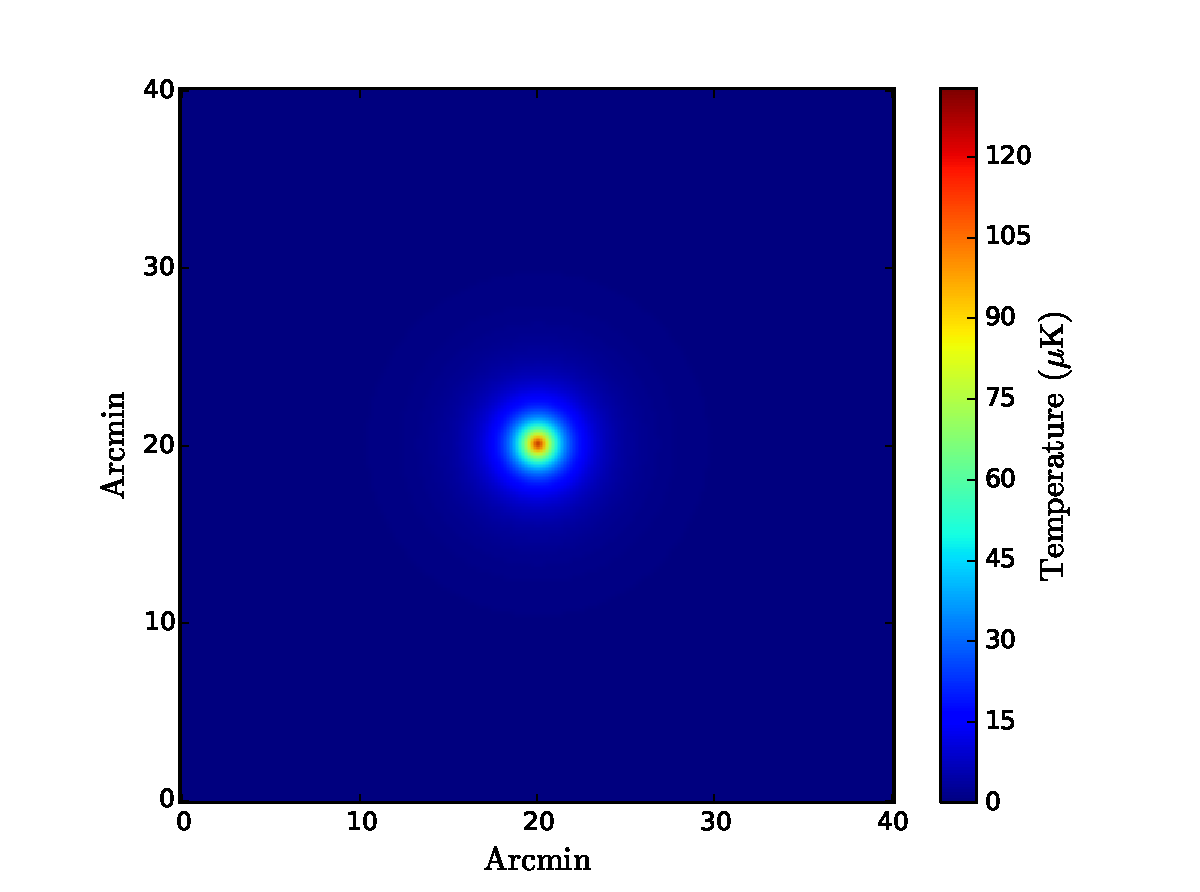
\includegraphics[scale=1.10, width=0.30\textwidth]{2.5_.22hm.pdf}
    }
    \hfill
    \subfloat[M = $3.5\times 10^{14} M_{\odot}$, Z= 0.22\label{subfig-2:dummy}]{%
      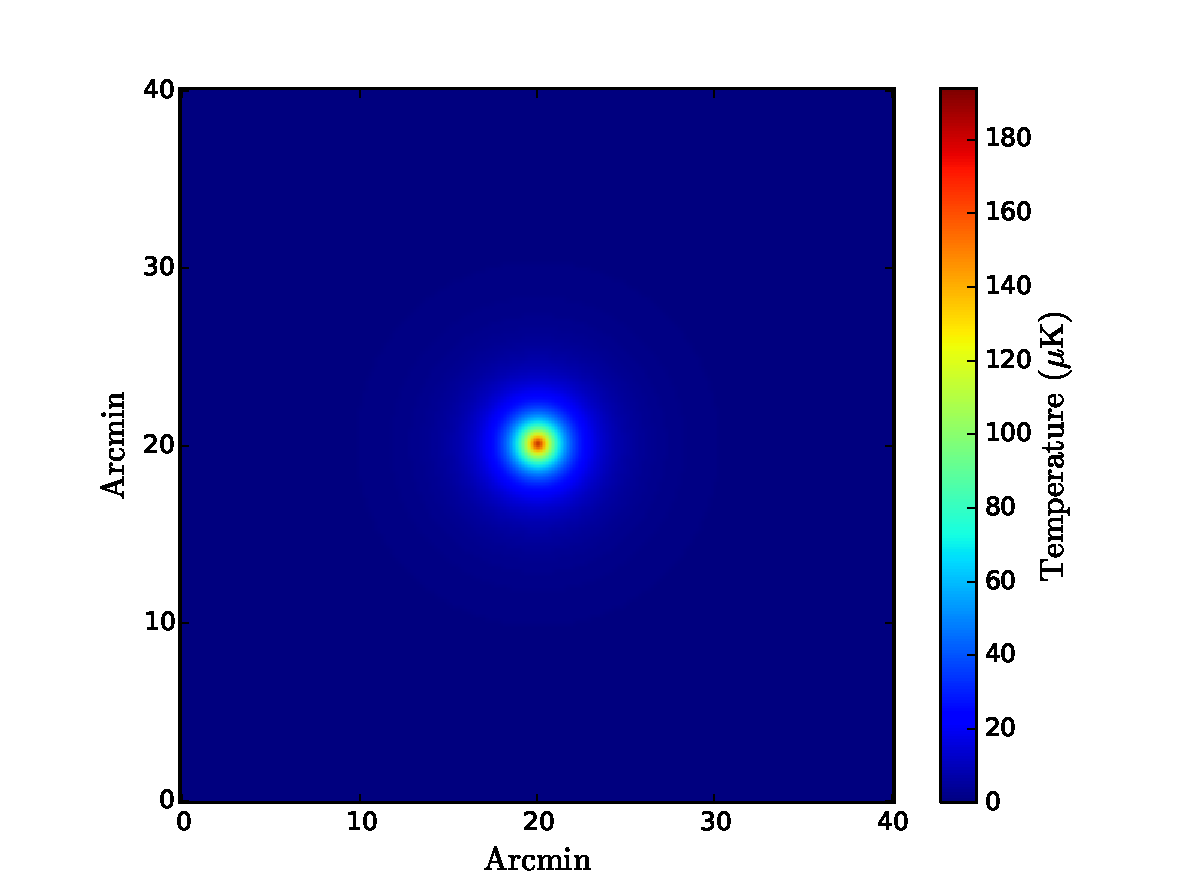
\includegraphics[scale=1.10, width=0.30\textwidth]{3.5_.22hm.pdf}
    }
    \hfill
    \subfloat[M = $4.5\times 10^{14} M_{\odot}$, Z= 0.22\label{subfig-2:dummy}]{%
      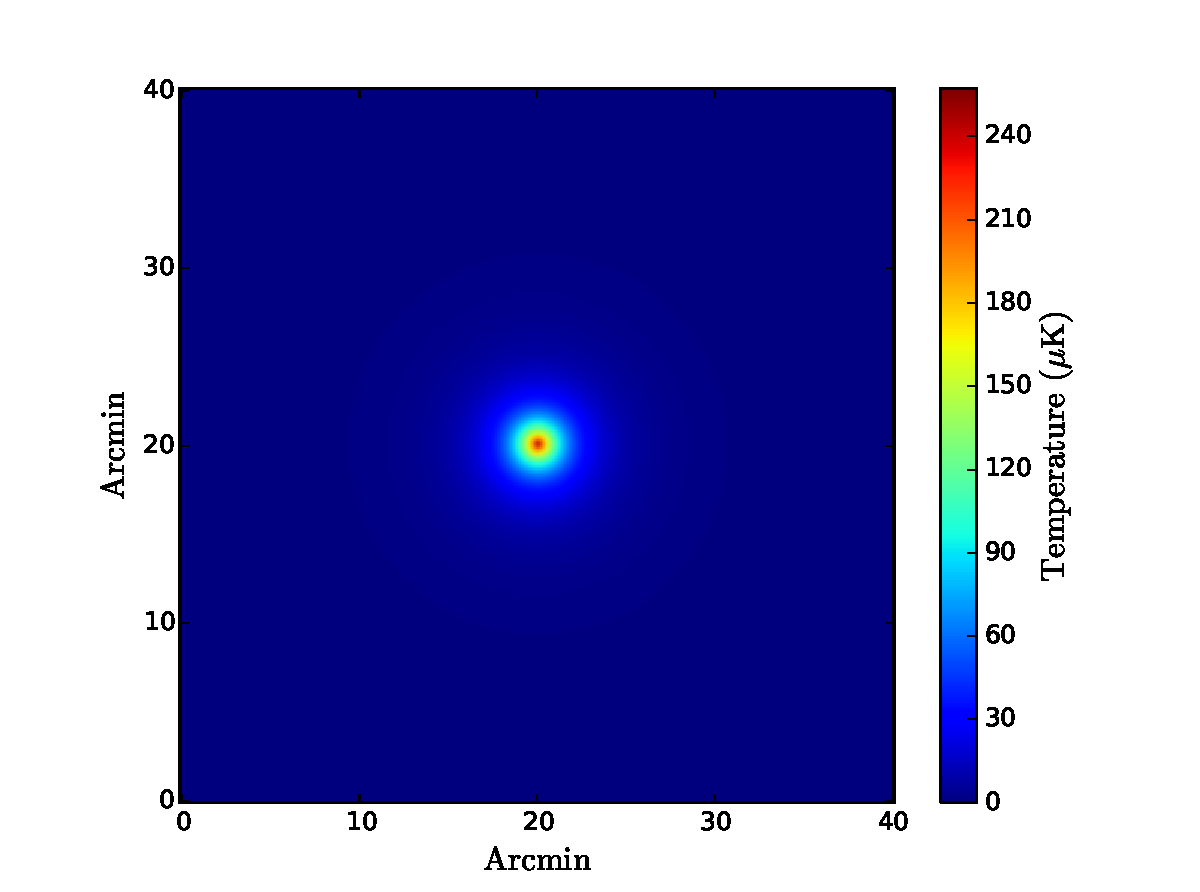
\includegraphics[scale=1.10, width=0.30\textwidth]{4.5_.22hm.pdf}
	}
    \vfill
    \subfloat[M = $2.5\times 10^{14} M_{\odot}$, Z= 0.55\label{subfig-2:dummy}]{%
      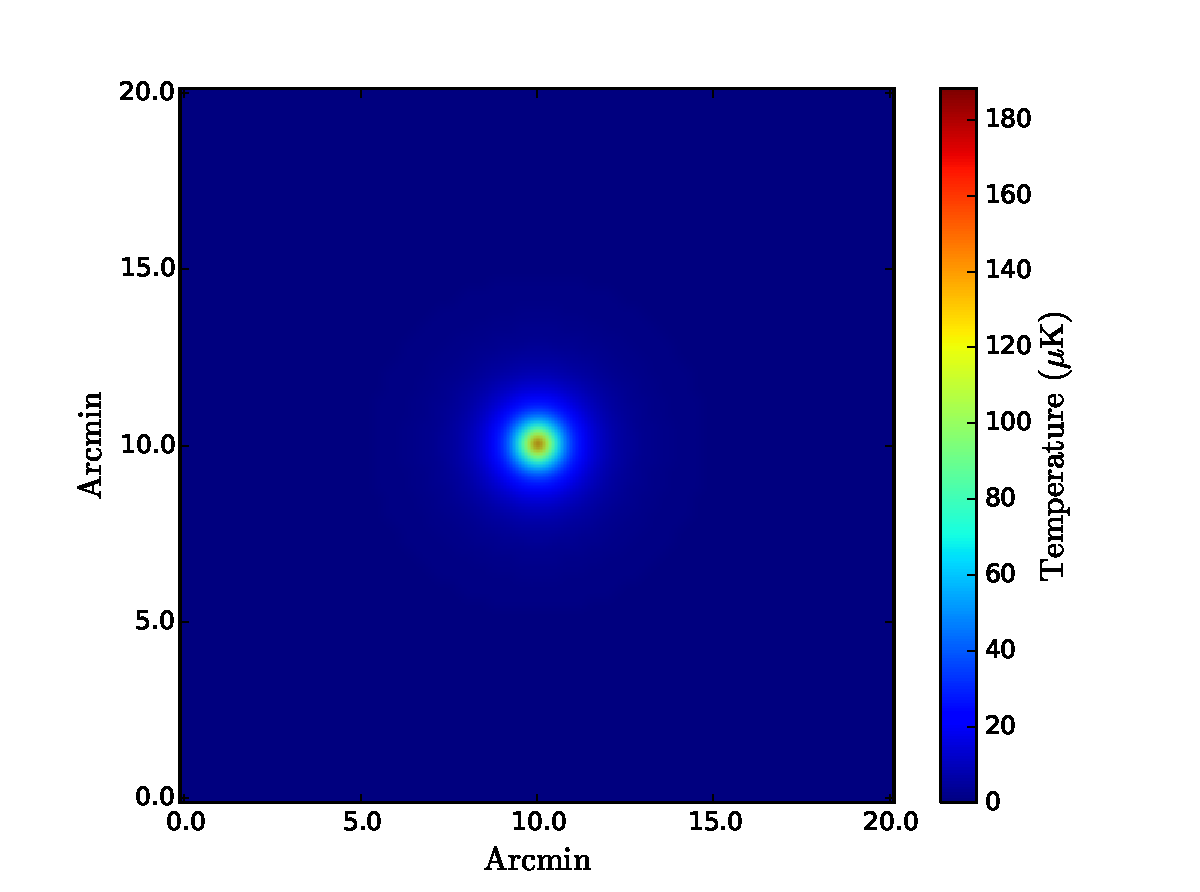
\includegraphics[scale=1.10, width=0.30\textwidth]{2.5_.55hm.pdf}
	}
    \hfill
    \subfloat[M = $3.5\times 10^{14} M_{\odot}$, Z= 0.55\label{subfig-2:dummy}]{%
      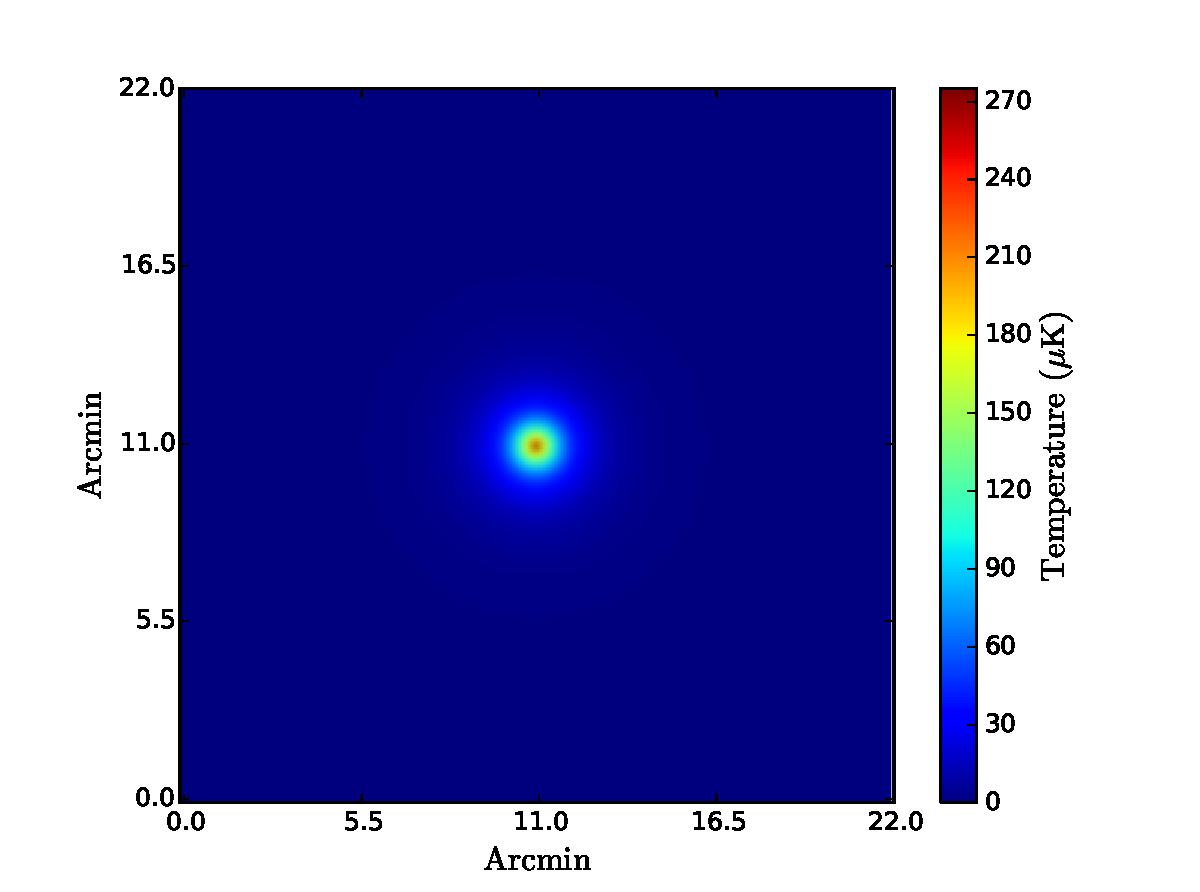
\includegraphics[scale=1.10, width=0.30\textwidth]{3.5_.55hm.pdf}
	}
    \hfill
    \subfloat[M = $4.5\times 10^{14} M_{\odot}$, Z= 0.55\label{subfig-2:dummy}]{%
      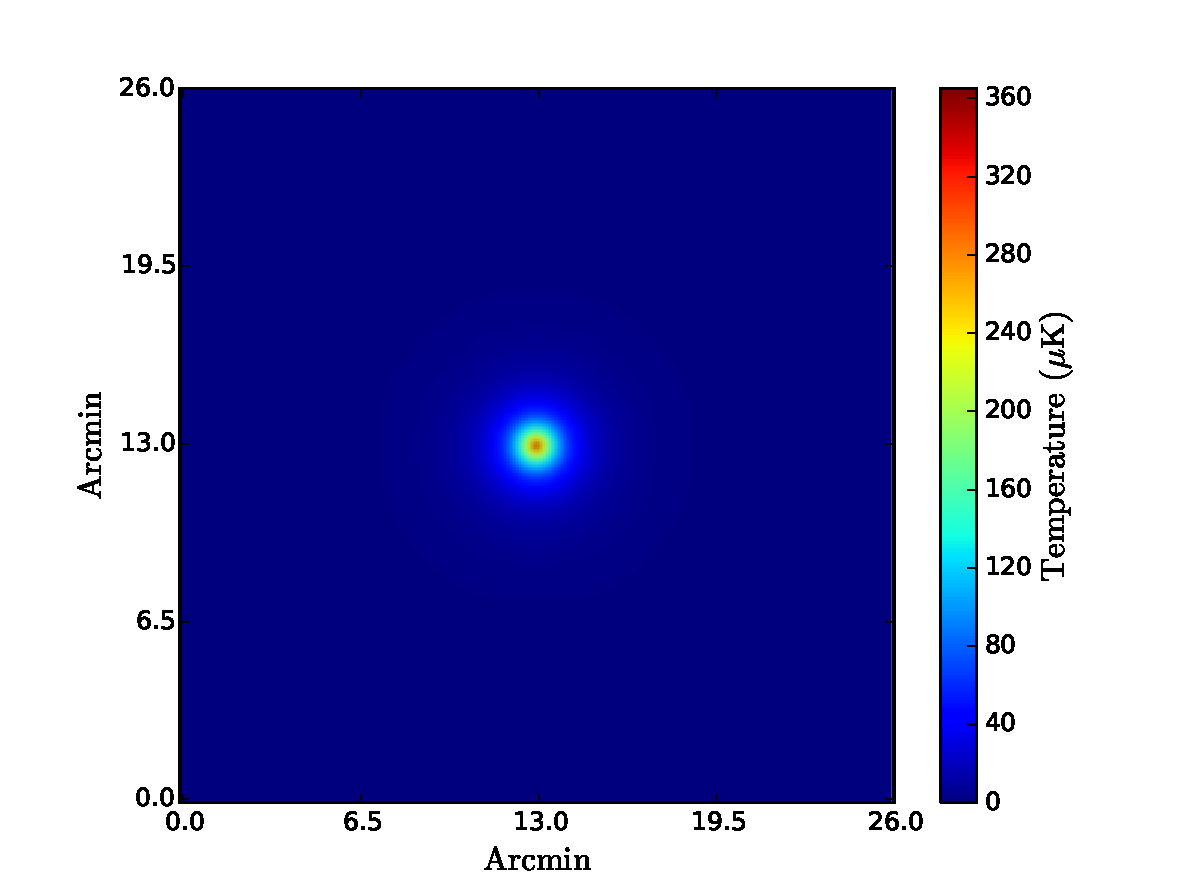
\includegraphics[scale=1.10, width=0.30\textwidth]{4.5_.55hm.pdf}
	}
    \vfill
    \subfloat[M = $2.5\times 10^{14} M_{\odot}$, Z= 1.00\label{subfig-2:dummy}]{%
      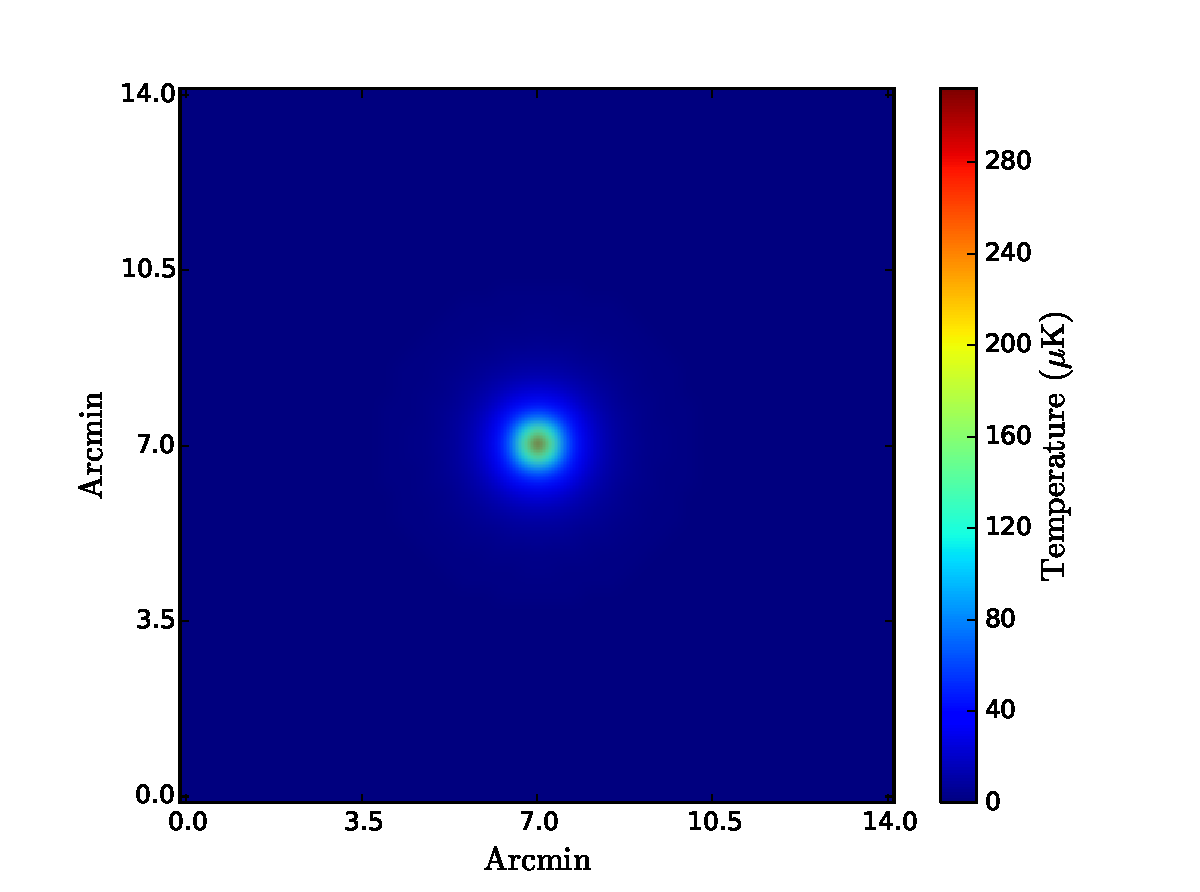
\includegraphics[scale=1.10, width=0.30\textwidth]{2.5_1hm.pdf}
	}
    \hfill
    \subfloat[M = $3.5\times 10^{14} M_{\odot}$, Z= 1.00\label{subfig-2:dummy}]{%
      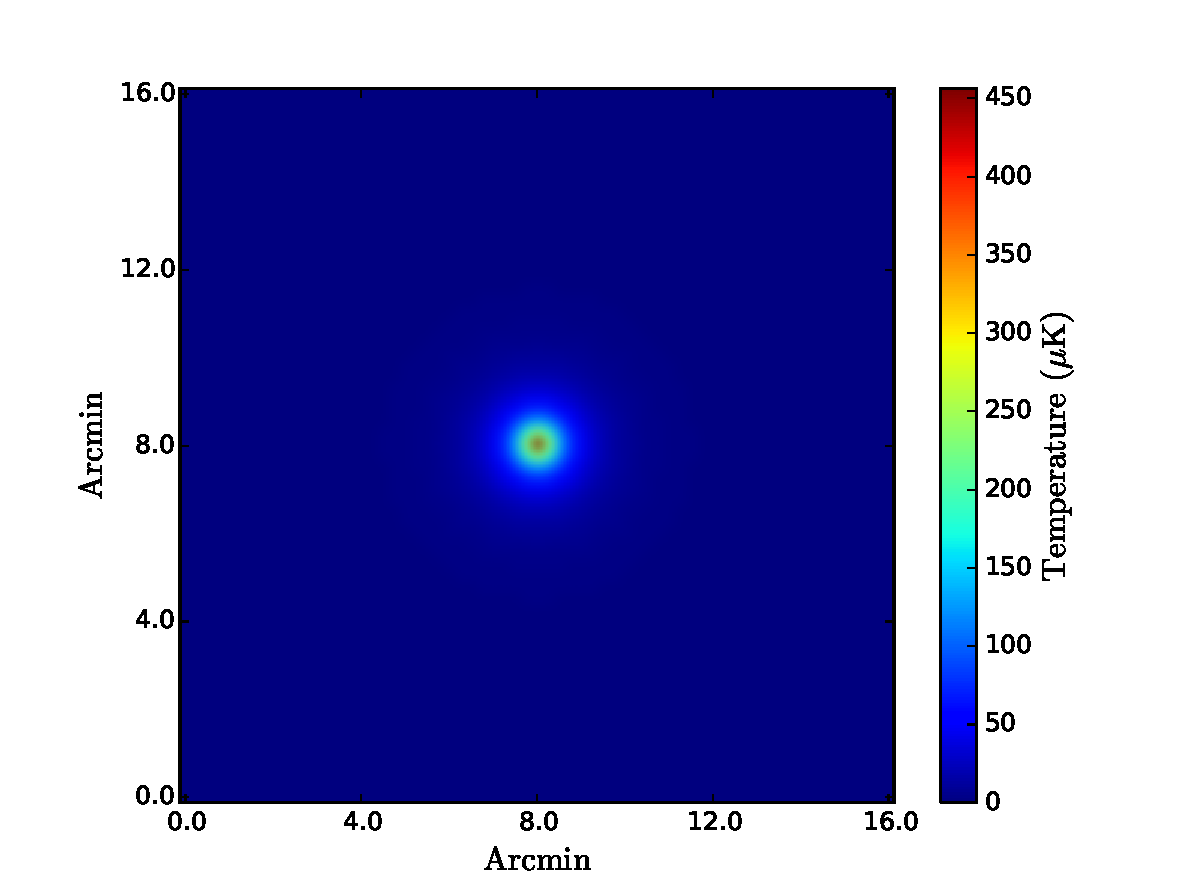
\includegraphics[scale=1.10, width=0.30\textwidth]{3.5_1hm.pdf}
	}
    \hfill
    \subfloat[M = $4.5\times 10^{14} M_{\odot}$, Z = 1.00\label{subfig-2:dummy}]{%
      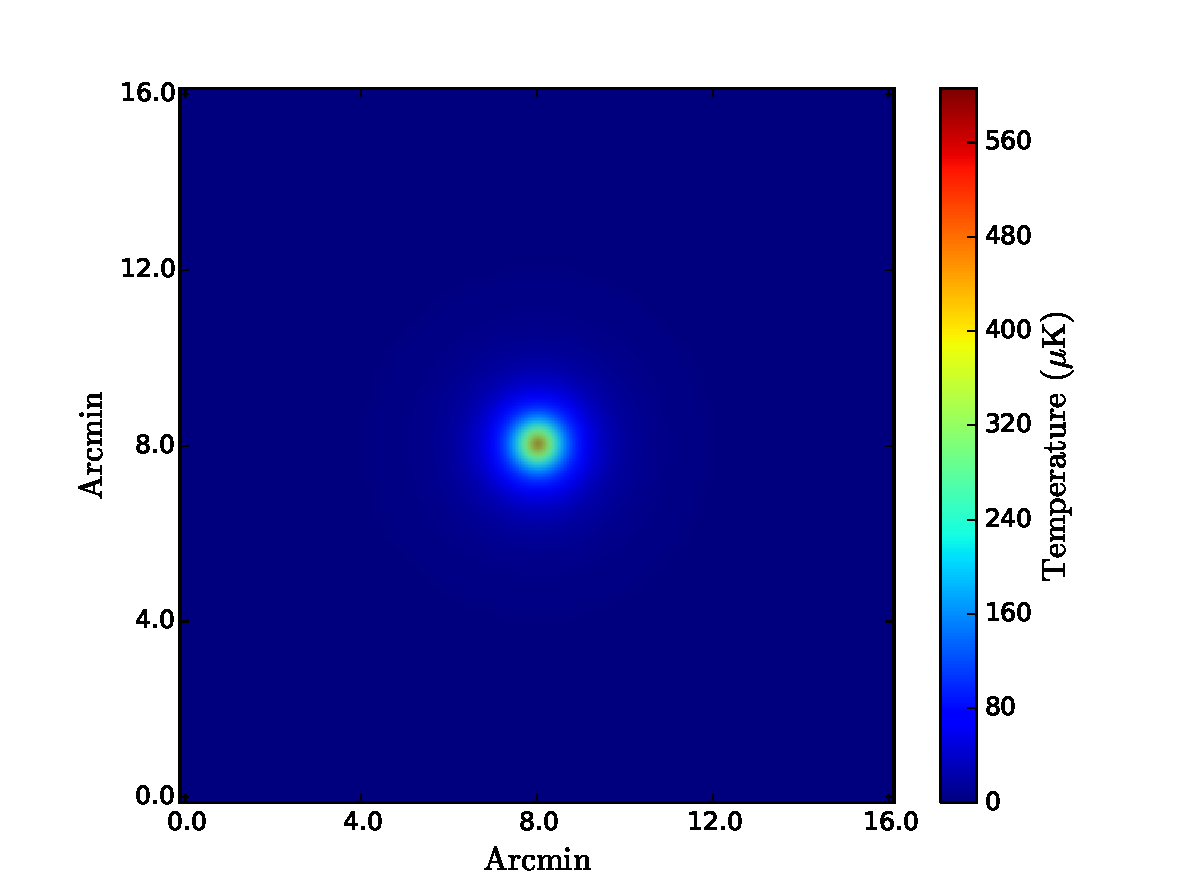
\includegraphics[scale=1.10, width=0.30\textwidth]{4.5_1hm.pdf}
	}
    \caption{Heat Maps Over Mass and Redshift Ranges}
    \label{fig:dummy}
  \end{figure}

\section{Discussion}

\end{document}
